\documentclass[twocolumn]{jarticle}

\usepackage{jsaiac}
\usepackage{graphicx}
\usepackage{amsmath}


%%
\title{
\jtitle{酒米:山田錦の倒伏シミュレーション}
\etitle{Simulation of Lodging in Sake Rice: Yamada Nishiki}
}
%%�p���͈ȉ����g�p
%\title{Style file for manuscripts of JSAI 20XX}

\jaddress{関西学院大学総合政策学部, 兵庫県三田市学園上ヶ原, ivk57020@kwansei.ac.jp}

\author{%
   \jname{星川 裕志\first{}}
   \ename{Yushi Hoshikawa}
\and
   \jname{山田 孝子\second{}}
   \ename{Takako Yamada}
%\and
%Given-name Surname\third{}%%�p���͍����g�p
}

\affiliate{
\jname{\first{}関西学院大学大学院総合政策研究科}%
\ename{Graduate School of Policy Studies, Kwansei Gakuin University}%
\and
\jname{\second{}関西学院大学総合政策学部メディア情報学科}
\ename{Department of Applied Informatics, School of Policy Studies, Kwansei Gakuin University}
%\and
%\third{}Affiliation \#3 in English%%�p���͍����g�p
}

%%
%\Vol{28}        %% <-- 28th�i�ύX���Ȃ��ł��������j
%\session{0A0-00}%% <-- �u��ID�i�K�{)

\begin{abstract}
   In modern rice farming, digital technology is used to collect growth data. The sake rice "Yamada Nishiki" has long stems and large grains, making it prone to lodging. This study developed a lodging simulation model considering stem strength and wind effects. The model reproduced lodging patterns observed in drone images and was used to evaluate the impact of factors such as stem strength and plant spacing on lodging. 
\end{abstract}

%\setcounter{page}{1}
\def\Style{``jsaiac.sty''}
\def\BibTeX{{\rm B\kern-.05em{\sc i\kern-.025em b}\kern-.08em%
 T\kern-.1667em\lower.7ex\hbox{E}\kern-.125emX}}
\def\JBibTeX{\leavevmode\lower .6ex\hbox{J}\kern-0.15em\BibTeX}
\def\LaTeXe{\LaTeX\kern.15em2$_{\textstyle\varepsilon}$}

\begin{document}
\maketitle

\section{はじめに}

\begin{figure}[bt]
    \centering
    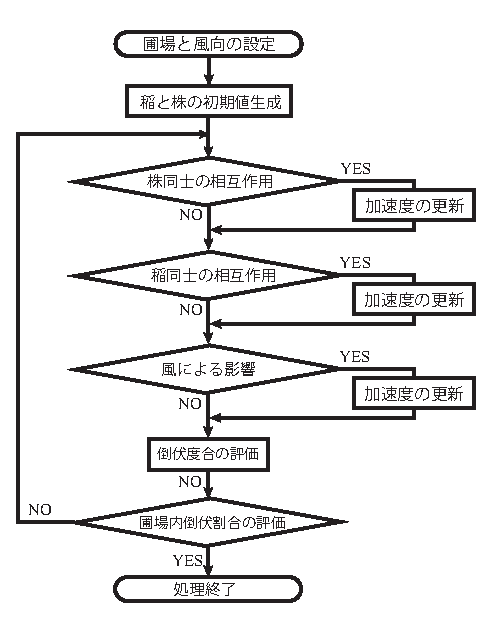
\includegraphics[width=0.8\linewidth]{fig/flow_figure.eps}
    \caption{シミュレーションの流れ}
    \label{fig:flow_figure}
\end{figure}

近年, 稲作の現場では省力化・労力軽減や生産性の向上, 生産物の品質向上のためデジタル技術の導入が様々な作物で検討されている\cite{inasaku-smart}. 
本研究ではドローン空撮で遭遇した稲穂が倒れる「倒伏」という現象をとりあげる.
倒伏は天候や稲穂の重みで稲が倒れる現象で, 稲穂が熟す8月末から収穫までに起こる. 倒伏した稲は品質低下をもたらすことで知られる.
本研究では兵庫県を代表する酒米「山田錦」を対象に,その倒伏メカニズムをシミュレーションでモデル化し, 倒伏に至る要素を検討し,空撮画像との特徴照合を行う.
山田錦は通常の稲に比べ, 大粒で草丈が約130cmと高く倒伏が起こりやすい品種として知られる\cite{yamadanishiki}.
食用米と異なり,酒米は栽培前に契約した買い手から品質と収量の確保が求められるので,「倒伏」は栽培上の重要な課題となっている.


\section{倒伏シミュレーションの設定}
本研究の倒伏シミュレーション全体構成を\ref{fig:flow_figure}に示す.
ここでは稲が倒れる過程の穂の角度に着目してモデル化する.
圃場内の各稲株は複数の茎からなり, 各茎の先端には稲穂がついている.
稲穂が風を受けて揺らぐと隣接する穂と接触し,接触の積み重ねが生む将棋倒しが圃場全体にわたり, 面的な倒伏に至る過程をモデル化する.

    \begin{enumerate}
    \item \label{item:setting} 圃場と風向の設定
    
    本シミュレーションでは稲株が存在する場となる圃場と風向が設定されているフローフィールドをそれぞれ別のものとして定義した.
    これは穂に対する風の作用が単調になることを防ぎ, より現実に即した形にするためである.
    まず, 圃場には$N \times N$株の稲株を株間$d_{s}$で等間隔に配置する.各稲株は予め半径$r_{3}$の円領域を持つとすると圃場の一辺$L$は
    \begin{eqnarray}
        L = d_{s} \times (N-1) + 2r_{3}\nonumber
    \end{eqnarray}
    となる.

    \begin{figure}[t]
        \centering
        \begin{minipage}{0.45\linewidth}
            \centering
            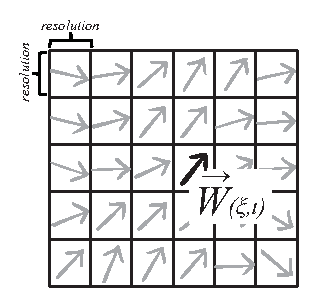
\includegraphics[width=\linewidth]{fig/flowfield.eps}
            \caption{フローフィールド}
            \label{fig:flowfield}
        \end{minipage}
        \hfil
        \begin{minipage}{0.45\linewidth}
            \centering
            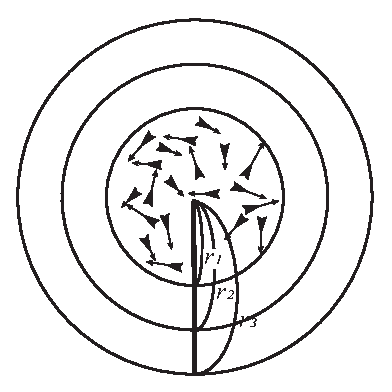
\includegraphics[width=0.8\linewidth]{fig/kabu_class.eps}
            \caption{稲株:単独の初期値}
            \label{fig:kabu_class}
        \end{minipage}
    \end{figure}
    
    \begin{figure}[t]
        \centering
        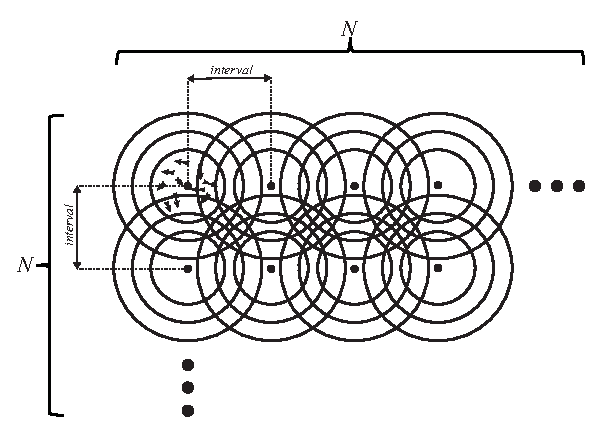
\includegraphics[width=\linewidth]{fig/hojo_class.eps}
        \caption{圃場内稲株と同心円領域}
        \label{fig:hojo_class}
    \end{figure}

    風はシミュレーション実行中, 格子領域(セル)ごとに与えた風力・方向で変わらずに吹くものとする.
    格子領域は解像度パラメータ$\rho$のとき、$L \times L$の圃場に$L/\rho$個のセル$(\xi,\iota)$単位で風向ベクトル$\vec{W}_{\xi,\iota}$を与える.
    風はパーリンノイズによる滑らかなランダム性を持つようにした.
    \ref{fig:flowfield}にその風向き例を示す.
    
    \item 稲株と稲穂の配置と設定
    
    一つの稲株$s_{i,j} \in S$は茎$k_{i,j,1} \sim k_{i,j,m}$を持ち, 茎の先端に稲穂$q_{i,j,1} \sim q_{i,j,m}$がつく.
    各株$s_{i,j}$は, 株中心から半径$r_1,r_2,r_3$,$(r_1<r_2<r_3)$の同心円の領域を持つものとする. 
    図\ref{fig:kabu_class}に示すように各稲株は$m=20$本の茎を持つものとする.各茎$k_{i,j,k}$は強度$f_{i,j,k}$, 茎長$h_{i,j,k}$で,
    茎強度$f_{i,j,k}$は$0\sim10$の範囲で与えるものとする.茎強度は確率分布に従って設定する.
    最初各茎先の穂の座標は半径$r_1$の円内にランダムに配置され, その向きも一様にランダムに与えられる.
    穂$q_{i,j,k}$は速度$v_{i,j,k}$, 加速度$a_{i,j,k}$を持つものとする.
    図\ref{fig:hojo_class}に圃場内の配置例を示す.
    

    \item 倒伏の段階的推移
    
    図\ref{fig:lodging-rad}に示す円の半径$r_1, r_2, r_3$の円内のどこに穂が位置するかに応じた倒伏度$D_{i,j,k}$を設定する.
    \begin{equation}
        D_{i,j,k} =
        \left\{
        \begin{alignedat}{3}
        1,\quad & \text{if }\quad d(q_{i,j,k}, C_{i,j}) \leq r_1 \\
        2, \quad & \text{if } \quad r_1 < d(q_{i,j,k}, C_{i,j}) \leq r_2 \\
        3, \quad & \text{if } \quad r_2 < d(q_{i,j,k}, C_{i,j}) \leq r_3
        \end{alignedat}\nonumber
        \right.
    \end{equation}
    
    間隔$d_s$で植えられた各株の中心座標$C_{i,j}$とし,それぞれの茎先には穂$q_{i,j,k}$がある.
    もし穂が$r_1$の円内に穂があればその茎の角度は$|\theta|<6/\pi$なので,ほぼ倒伏がない状態に対応する.同様に穂の位置が$r_1$の円を超えて$r_2$の円内にあるときは,茎の角度は$\pi/6<|\theta|\le\pi/3$, 半径$r_3$なら茎の角度は$\pi/3<|\theta|\le\pi/2$と想定され,倒伏が進行した状態となる.
    
    \begin{figure}[t]
        \centering
        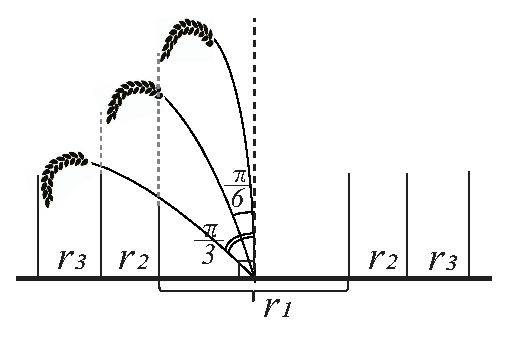
\includegraphics[width=0.8\linewidth]{fig/lodging-rad.eps}
        \caption{倒伏度}
        \label{fig:lodging-rad}
    \end{figure}

    \end{enumerate}


    \subsection{倒伏シミュレーション:穂の位置の更新} \label{section:update}
    シミュレーションは時刻$0 \sim n$まで時点単位で進行する. 各稲穂は, 各株・稲穂同士による相互作用や風による影響で時点$t$の状態から,次時点$t+1$の状態に推移する.各時点ですべての稲穂に述べる単純なルールを適用して状態(穂の位置)を更新する手続きをおこない,その繰り返しでシミュレーションは進行する.
    時刻$t$での更新は稲株$s_{i,j}$として,まず$s_{1,1}, s_{1,2}, \dots, s_{1,N}$から始まり, 次に$s_{2,1}, s_{2,2}, \dots, s_{2,N}$に進み,
    最終的には$s_{N,N}$までの順に行い,全部終わると次時刻$t+1$に進む.
    各稲株$s_{i,j}$内ではその下部に属す穂$q_{i,j,k}$はランダムに選ばれ順に更新される. 
    穂の位置を更新する要素としては速度$\mathbf{v}_{i,j,k}$と
    加速度$\mathbf{a}_{i,j,k}$がある.更新の際にはそれぞれ上限値$U_s, U_f$を予め設定して与える. 


    % \subsubsection{株同士の相互作用}

    % \begin{description}
    %     \item{step1.} 株$A,B$に含まれる穂の座標から株$A$,株$B$の重心を求める
    %     \item{step2.} 株$A,B$に属する穂から,重心からの距離が閾値以下の穂の集合$A*,B*$を抽出する(抽出された穂は相互に株間で接触したとみなす)
        
    %    \item{step3.} 抽出された穂の集合$A*,B*$の平均速度ベクトル$\bar{\boldsymbol{v}}_{i,j,k\in A*}$,$\bar{\boldsymbol{v}}_{i,j,k\in B*}$を求める. (平均速度ベクトルを図中の破線の矢線で表す)
    %     \item{step4.} $maxV_{AB}=max(\|\bar{\boldsymbol{v}}_{i,j,k\in A*}$,$\bar{\boldsymbol{v}}_{i,j,k\in B*})$を求める. (この例では$maxV_{AB}=\bar{\boldsymbol{v}}_{i,j,k\in B*}$)
        
    %     \item{step5.} $A$株の速度ベクトル$Q_{A}=maxV_{AB}$とする
    %     \item{step6.} 株$A$に含まれる穂$q_{i,j,k \in A}$について以下を計算する
        
    %     \item{(6-1).} 穂$q_{i,j,k \in A}$の位置ベクトル$\gamma_{i,j,k \in A}$とすると,
    %         次時点の穂の位置は\[\gamma_{i,j,k \in A}^{\prime}=\gamma_{i,j,k \in A}\frac{maxV_{AB}}{\|maxV_{AB}\|}\]
    %     \item{(6-2).} $\bar{o}_{i,j,k \in A}=(q_{i,j,k \in A})×1/f_{i,j,k \in A}$を計算する
    %     \item{(6-3).} 操舵力$l_{i,j,k\in A}=v_{i,j,k \in A}-\bar{O}_{i,j,k \in A}$を計算する
    %     \item{(6-4).} 穂の加速力$a_{i,j,k \in A}=q_{i,j,k \in A}$を更新する
        

    % \end{description}


    %         \begin{figure}[tbp]
    %             \centering
    %            \includegraphics[width=0.8\linewidth]{figure/kabus.eps}
    %             \caption{株同士の相互作用}
    %             \label{fig:kabus}
    %         \end{figure}

    \subsubsection{株同士の相互作用}
    ここでは図\ref{fig:kabus}に示す2株$A,B$を例に述べる.
    \begin{description}
        \item{step 1.} いま株$A$が座標$C_(i,j)$にあるとき,$A$の3つ先までの隣接株(ただし株$A$を除く)について,その穂の座標から各株の重心を求める.
        \item{step 2.} 株$A$の重心座標$g_{i,j}$からの距離が閾値$\lambda$以下の株の集合$S_{adj}$を抽出する(例では株$B$のみ抽出された場合).
        \item{step 3.} 株$A$と抽出された株$B$に属する穂集合の平均速度ベクトルを\\
        $\displaystyle \bar{\mathbf{V}}_{A}=1/|A|{\sum_{A} \mathbf{v}}$,\\
        $\displaystyle \bar{\mathbf{V}}_{B}=1/|B|{\sum_{B} \mathbf{v}}$\\
        とする. (破線で示される矢線)
        \item{step 4.} $\displaystyle\mathbf{maxV}_{AB}=\rm{max}(\bar{\mathbf{V}}_{A},\bar{\mathbf{V}}_{B})$とする.
        %例では\\
        %$\displaystyle %\mathbf{maxV}_{AB}=\bar{\mathbf{V}}_{B}$となる.
        \item{step 5.} $A$株への作用ベクトルを$\displaystyle\mathbf{O}_{A}=\mathbf{maxV}_{AB}$とする. 
        \item{step 6.} 株$A$の穂$q_{i,j,k \in A}$が受ける作用ベクトル$\mathbf{o}_{i,j,k \in A} \\
        =\mathbf{O}_{A}(f_{i,j,k})^{-1}$とする.
        \begin{description}
            % \item{(6-1)} 次時点の穂の位置$\gamma_{i,j,k \in A}^{\prime}=\frac{\mathbf{maxV}_{AB}}{\|\mathbf{maxV}_{AB}\|}\gamma_{i,j,k \in A}$
            % \item{(6-2)} 次時点の穂の速度 $\mathbf{v}_{i,j,k \in A}^{\prime}=\mathbf{v}_{i,j,k \in A}\cdot f_{i,j,k \in A}^{-1}$
            \item{(6-1)} 操舵力を求める$\mathbf{l}_{i,j,k\in A}=\mathbf{o}_{i,j,k \in A}-\mathbf{v}_{i,j,k \in A}$
            \item{(6-2)} 加速度$\mathbf{a}_{i,j,k}$の更新$\mathbf{a}^{(kabu)\prime}_{i,j,k \in A}=\mathbf{a}_{i,j,k \in A}+\mathbf{l}_{i,j,k \in A}$
        \end{description}
    \end{description}

    %\begin{description}
    %\item{step1.} 株$A,B$の穂の座標$\gamma_{i,j,k \in A}$からは株$A$の重心,$\gamma_{i,j,k \in B}$からは株$B$の重心を求める
    %\item{step2.}それぞれの株について,重心からの距離が閾値$\lambda$以下の穂の集合$A^{*},B^{*}$を抽出(抽出された穂は株間で接触したとみなす)
    %\item{step3.} 抽出された穂の集合$A^{*},B^{*}$の平均速度ベクトル
    %    $\displaystyle \bar{\mathbf{V}}_{A^{*}}=1/|A|\sum_{\bar{\mathbf{v}}_{A^{*}}} \mathbf{v}$,
    %    $\displaystyle \bar{\mathbf{V}}_{B^{*}}=1/|B|\sum_{\bar{\mathbf{v}}_{B^{*}}} \mathbf{v}$,
    %    とする. (図中の破線矢線)
    %\item{step4.} $\displaystyle\mathbf{maxV}_{AB}=\rm{max}(\mathbf{v}_{i,j,k\in A^{*}}$,$\mathbf{v}_{i,j,k\in B^{*}})$とする.
    %    例では$\displaystyle \mathbf{maxV}_{AB}=\mathbf{v}_{i,j,k\in B^{*}}$
    %\item{step5.} $A$株への作用ベクトル$\displaystyle\mathbf{O}_{A}=\mathbf{maxV}_{AB}$とする
    %\item{step6.} 株$A$の穂$q_{i,j,k \in A}$の受ける作用ベクトル$\mathbf{o}_{i,j,k \in A}=\mathbf{O}_{A}(f_{i,j,k})^{-1}$とする
    %    \begin{description}
    %    \item{(6-1)} 次時点の穂の位置$\gamma_{i,j,k \in A}^{\prime}=\frac{\mathbf{maxV}_{AB}}{\|\mathbf{maxV}_{AB}\|}\gamma_{i,j,k \in A}$
    %    \item{(6-2)} 次時点の穂の速度 $\mathbf{v}_{i,j,k \in A}^{\prime}=\mathbf{v}_{i,j,k \in A}\cdot f_{i,j,k \in A}^{-1}$
    %    \item{(6-3)} 次時点の穂の操舵力$\mathbf{l}^{\prime}_{i,j,k\in A}=\mathbf{o}_{i,j,k \in A}-\mathbf{v}_{i,j,k \in A}$
    %    \item{(6-4)} 次時点の穂の加速力$\mathbf{a}^{(kabu)\prime}_{i,j,k \in A}=\mathbf{a}_{i,j,k \in A}+\mathbf{l}_{i,j,k \in A}$
    %    \end{description}
    %\end{description}
                \begin{figure}[tbp]
                    \centering
                   \includegraphics[width=0.8\linewidth]{fig/kabus.eps}
                    \caption{株同士の相互作用}
                    \label{fig:kabus}
                \end{figure}

        \subsubsection{穂同士の相互作用}

        \begin{figure}[t]
            \centering
            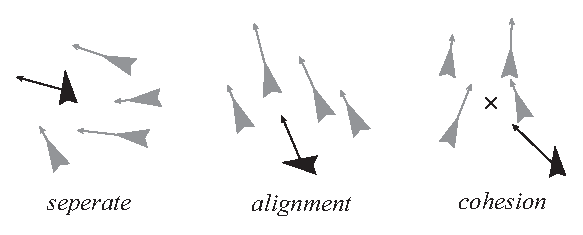
\includegraphics[width=\linewidth]{fig/flocking.eps}
            \caption{穂群の動き}
            \label{fig:flocking}
        \end{figure}

        株内の穂の相互作用, 分離・整列・凝集の3つのルールを順次適用し状態を更新する. 稲株$A$に属する任意の穂$q_{i,j,k \in A}$について以下の処理を行う. \\
        \begin{itemize}
            \item 分離\\
            %\noindent{\bf 分離}\\
                株内の他の穂と衝突を避ける動きを表す.株$A$から任意に選んだ穂$q_{i,j,k \in A}$に対し一定距離$d_{\nu}$内にある他の株との間のベクトル$\hat{\mathbf{\nu}}_{i,j,k^{\prime} \rightarrow k}$を正規化する.
            \begin{description}
                \item{step1.}
    $\hat{\mathbf{\nu}}_{i,j,k^{\prime} \rightarrow k} =$  
    $\frac{\gamma_{i,j,k \in A} - \gamma_{i,j,k^{\prime} \in A}}
    {\|\gamma_{i,j,k \in A} - \gamma_{i,j,k^{\prime} \in A}\|}$
    
    %$\{ \gamma_{i,j,k \in A} - \gamma_{i,j,k^{\prime} \in A }\\ \quad \quad |k^{\prime} \neq k ,\|\gamma_{i,j,k \in A} %- \gamma_{i,j,k^{\prime} \in A} \| \leq d_{s}\}$\\

                \item{step2.} 次に穂間の距離の逆数で重みづけした平均ベクトルを求める.ただし, $N$は$d_{\nu}$内の株の総数,$D_{\nu}$は$k$を除く同じ稲に属する距離$d_{\nu}$内の稲穂の集合で$\|\gamma_{i,j,k} - \gamma_{i,j,k^{\prime}} \| \leq d_{\nu}$を満たす.
        \[
        \overline{\mathbf{\nu}}_{i,j,k} = \frac{1}{N} \sum_{D_{\nu}}{\frac{\hat{\mathbf{\nu}}_{i,j,k^{\prime} \rightarrow k}}{\|\gamma_{i,j,k \in A} - \gamma_{i,j,k^{\prime} \in A}\|}}
        \]

        \item{step3.} 正規化しスケール係数 $U_s$を乗じる.\\
            $\mathbf{M}_{\nu}=U_{s} \frac{\bar{\mathbf{\nu}}_{i,j,k}}{\|\bar{\mathbf{\nu}}_{i,j,k}\|}$
            \item{step5.} 操舵力ノルムの上限を \( U_f \) として次時点の操舵力を計算する.
            \[\mathbf{l}_{i,j,k}^{(sep)\prime}=min(U_{f}, \hat{M}_{\nu}-\mathbf{v}_{i,j,k} ) \]
            \end{description}
        \item 整列\\
        %\noindent{\bf 整列}\\
            整列はお近隣の穂と同じ方向に進む作用をする.計算手続きは「分離」と同様であるが,穂間の距離の逆数で重みづけしない平均速度ベクトルで計算する.
            ただし, $D_{\psi}$は$k$を除く同じ稲に属する距離$d_{\psi}$内の稲穂の集合で$\|\gamma_{i,j,k} - \gamma_{i,j,k^{\prime}} \| \leq d_{\psi}$を満たす.
            %$Ds^{\prime}$はを$k' \neq k, \|\gamma_{i,j,k \in A} - \gamma_{i,j,k' \in A} \|$としたとき,
            \[
            \overline{\mathbf{\nu}}_{i,j,k} = \frac{1}{N} \sum_{D_{\psi}} {v}_{i,j,k'}
            \]
            とする.
        \item 凝集\\
        %\noindent{\bf 凝集}\\
        計算手続きは「分離」と同じだが$\nu_{i,j,k^{\prime} \rightarrow k}, D_{\nu}$の代わりに$\nu_{i,j,k \rightarrow k^{\prime}}, D_{\psi}$用いて計算する.
        \item 加速度更新\\
        %\noindent{\bf 加速度更新}\\        
        予め与えた重み$\omega_s, \, \omega_a, \, \omega_c$と株間で求めた次時点の加速度から次時点の穂の加速度を更新する
                \[
                    \mathbf{a}^{\prime}_{i,j,k} = \mathbf{a}^{(kabu)\prime}_{i,j,k} +\omega_s  \mathbf{l}_{i,j,k}^{(sep)\prime} +\omega_a \mathbf{l}_{i,j,k}^{(ali)\prime}+\omega_c  \mathbf{l}_{i,j,k}^{(coh)\prime}
                \]

        \end{itemize}


        \subsubsection{風の影響}
        %\noindent{\bf 風の影響}\\
        まず穂$q_{i,j,k}$は穂の位置に対応するセルを参照する.該当するセルの風向単位ベクトル$\vec{w}_{ix,iy}$,速度ベクトルの上限を$U_{s}$とすると,風の影響を加味した次時点の操舵力は次のように計算され,$\mathbf{l}_{i,j,k}^{\prime\prime}$と加速力$\mathbf{a}_{i,j,k}^{\prime\prime}$が得られる.
        \[
        \mathbf{l}_{i,j,k}^{\prime\prime}=min(U_{f},\frac{U_{s}}
        {f_{i,j,k}} \vec{W}_{ix,iy} -\mathbf{v}_{i,j,k}^{\prime})
        \]
        \[
        \mathbf{a}_{i,j,k}^{\prime\prime}= \mathbf{a}_{i,j,k}^{\prime}+\mathbf{l}_{i,j,k}^{\prime}
        \]

        \subsubsection{穂の位置の更新}
        %\noindent{\bf 穂の位置の更新}\\
        時点$t$における穂$q_{i,j,k,t}$の位置から次時点の時刻$t+1$の位置は,
        \[   
            \mathbf{\gamma}_{i,j,k}^{t+1} = \mathbf{\gamma}_{i,j,k}^{t} + \mathbf{v}_{i,j,k}^{\prime} + \mathbf{a}^{\prime\prime}_{i,j,k}
        \]
        となる.

        \subsection{倒伏度の更新}
        %\noindent{\bf 倒伏度の更新}
        穂の位置が円$r_1$内から円$r_2,r_3$が作る領域に移行するにつれて,倒伏度$D_{i,j,k}$を変更する.倒伏の進行は不可逆とする. 

        \subsection{終了判定}
        %\noindent{\bf 終了判定}
        あるしきい値$\gamma_{end}$を予め設定し,\\
        \[
            \frac{1}{mN^{2}}\sum_{q_{i,j,k} \, | \, D_{i,j,k}=3}{1}\ge \gamma_{end} 
        \]
        となったとき,圃場全体が一定レベルで倒伏したと判定してシミュレーションを終了する. 
        終了しない場合は上記の手続きを株,株内の穂に対して続け,処理を繰り返す.
        % $\sum_{i} \sum_{j} \sum_{k} \mathbf{1}(D_{i,j,k} = 3)/mN^{2} \ge \gamma_{end}$

        \begin{table}[b]
            \begin{tabular}{||l|l||}
                \hline
                一辺の株数$N$ & 30 \\  \hline
                株間距離$d_s$ &20 \\ \hline
                風向場の解像度 $\rho$&20 \\ \hline
                稲穂領域 $r_1$ & 30 \\ \hline
                茎本数  $m$& 20 \\ \hline
                茎長 $h_{kij}$& 120 \\\hline
                茎強度 $f_{i,j,k}$ &$\sim \mathcal{N}( 5, 5/3)$\\\hline
                速度ベクトル上限$U_{s}$&1.0\\\hline
                加速度ベクトル上限$U_f$&0.3 \\ \hline
                %倒伏しきい値 ($\lambda_1,\lambda_2$)&(0.54,0.63) \\ \hline
                穂の相互作用の重み ($\omega_s,\omega_a,\omega_c)$&(0.6,0.1,0.3) \\ 
                \hline
                終了判定しきい値  $\gamma_{end}$&50 \\\hline
            \end{tabular}
            \caption{シミュレーション・パラメータ}
            \label{table:standards}
        \end{table}
        \begin{table}[bt]        
            \begin{tabular}{|c|c|c|c|}
                \hline
                実験 & 操作変数 & 設定範囲 & 刻み幅 \\
                \hline
                実験1 & $\mu$ & $0\sim10$ & 0.1 \\
                \hline
                実験2 & $H$ & $80\sim160$ & 1 \\
                \hline
                実験3 & $I$ & $0\sim100$ & 1 \\
                \hline
            \end{tabular}  
            \caption{実験の設定} 
            \label{table:jikken}
        \end{table}


\section{実験}
シミュレーションの設定パラメータを表\ref{table:standards}に示す. 
実験はシミュレーション終了までの繰り返し処理回数(時刻)に対する, 実験1「茎強度」, 実験2「茎長」, 実験3「株間の距離」を調べた.各実験の変数設定を\ref{table:jikken}に示す.各設定毎に100回ずつ実施して平均, 標準偏差を求めた.

\section{結果}
%\noindent{\bf 実験}
実験の結果を図\ref{fig:e1}, \ref{fig:e2}, \ref{fig:e3}に示す. 横軸にそれぞれ茎強度生成の正規分布の平均$\mu$, 茎の高さ$h$, 株間距離$d_s$をとり, 縦軸には圃場内の一定比率の穂が倒伏するまでの時間を示す.
実験1では圃場内の茎が強度があがれば倒伏が起きにくく, 広がりにくいことを示唆している.
実験2,3の結果は紙面都合で発表時に譲る.

%\noindent{\bf シミュレーション画面と空撮画像}
次に本シミュレーション画像を実際の圃場のドローン空撮画像を図\ref{fig:disp1}に示す.倒伏に特徴的なうねり模様が両方の図で見られる.
%定量的な部分は今後の課題として残されている. 本シミュレーションの結果画像と実際の圃場の空撮画像を比較し, 画像処理による倒伏の割合の評価を行うことで, シミュレーションの妥当性を定量的に検証する予定である.



%$%実験1の結果を\ref{fig:e1}に示す. 横軸には操作変数の値を標準化したものを, 縦軸には\ref{fig:flow_figure}のループ部を1時点とした場合の経過時点数を示している. 実験1では$\mu$が高くなるほど倒伏に至る時間が長くなることが分かった. つまり, 圃場内の茎が強い稲が多くなるほど倒伏が起きにくく, 広がりづらいということを示している. 実験2では, $H$の値の変化に対して倒伏至る時間が変化することはなく, 一定の値であった. 茎の高さは稲1本の倒伏のしやすさには強く影響するかもしれないが, それらを群としてみたときにはそこまで倒伏に至る時間に影響を及ぼさない要素だと考察する. 実験3では, 最初は$I$が大きくなるにつれて急激に倒伏に至る時間も大きくなったが, $I$が40くらいを超えるとそこから倒伏までの時間は一定の値をとるようになることが分かった. $I=40$のときはまだ株の倒伏範囲$r_1$に重なりがあり, 完全に株が独立するようになったわけではない. 株間距離は大きくすればするほど倒伏しにくくなるというわけではなく, ある距離からはそれ以上大きくしても意味がないということがいえる. このある距離がどのようにして決まっているのかを明らかにするため, より詳細な検証が必要である. 


% \begin{figure}[tb]
%     \begin{minipage}{0.5\linewidth}
%         \centering
%         \includegraphics[width=\linewidth]{figure/e1.eps}
%         \caption{実験1}
%         \label{fig:e1}
%     \end{minipage}
%     \begin{minipage}{0.5\linewidth}
%         \centering
%         \includegraphics[width=\linewidth]{figure/e3.eps}
%         \caption{実験3}
%         \label{fig:e3}
%     \end{minipage}
% \end{figure}



\section{まとめと今後の課題}
本実験では, 稲穂と稲穂の接触の積み重ねから面的に倒伏が広がる状況をモデル化し, シミュレーションを行った. 
今後の課題は,大きく二つある.一つは様々なシミュレーションの変数設定で,倒伏に影響する要素の検討である.
二つ目は倒伏シミュレーション結果とドローン空撮による倒伏画像の比較からシミュレーションの妥当性を
定量的に検証することである.


\begin{thebibliography}{99}
\bibitem[南石 19]{inasaku-smart}
南石 晃明: 稲作スマート農業の実践と次世代経営の展望, 養賢堂, 2019
\bibitem[兵庫酒米研究グループ 10]{yamadanishiki}.
兵庫酒米研究グループ: 山田錦物語 : 人と風土が育てた日本一の酒米, 神戸新聞総合出版センター, 2010.
\bibitem[永井 21]{yoshi-1}
永井拓生: ヨシの力学的特性に関する基礎的研究 その1 ヨシ稈の形状および曲げに対する力学的特性, 日本建築学会大会学術講演梗概集(東海), 2021.
\bibitem[永井 21]{yoshi-2}
永井拓生: ヨシの力学的特性に関する基礎的研究 その1 ヨシ稈の形状および曲げに対する力学的特性, 日本建築学会大会学術講演梗概集(東海), 2021.
\bibitem[Shiffman 14]{noc}
Daniel Shiffman: Nature of Code: Processingではじめる自然現象のシミュレーション, ボーンデジタル, 2014.
\end{thebibliography}

\begin{figure}[b]
    \centering
    \includegraphics[width=\linewidth]{fig/e1.eps}
    \caption{実験1}
    \label{fig:e1}
\end{figure}

\begin{figure}[tb]
    \centering
    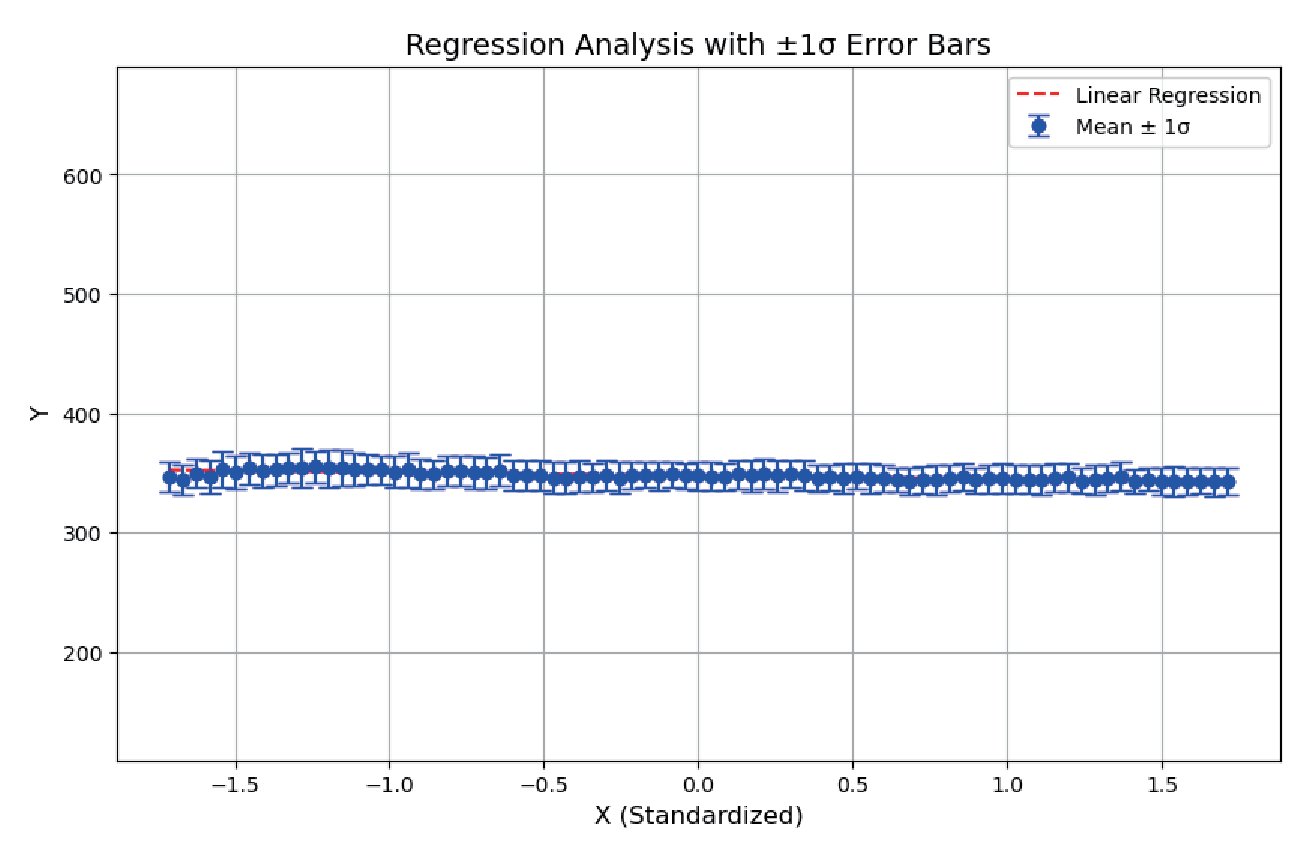
\includegraphics[width=\linewidth]{fig/e2.eps}
    \caption{実験2}
    \label{fig:e2}
\end{figure}

\begin{figure}[tb]
    \centering
    \includegraphics[width=\linewidth]{fig/e3.eps}
    \caption{実験3}
    \label{fig:e3}
\end{figure}

\begin{figure}[tb]
    %\left
    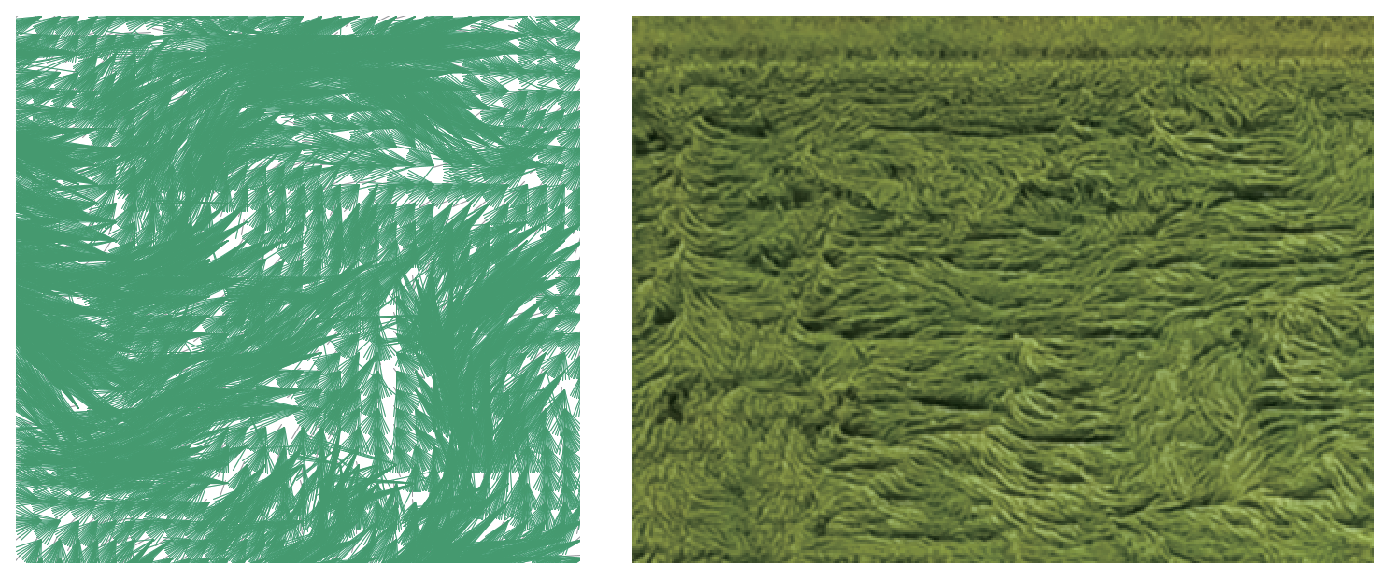
\includegraphics[width=\linewidth]{fig/comparison.eps}
    \caption{実験画像と空撮画像}
    \label{fig:disp1}
\end{figure}
%%

\end{document}
